\chapter{Implementation}

\textbf{Author: } 

\section{Generating test data}
Good test data is of utmost importance in machine learning. The system can only know information that is depicted in the training data, which is why it is important to include as many aspects of the problem as possible in this data.

Since machine learning needs a lot of data in order to solve the given task it can be tiresome to generate and label all this data by hand. Therefore the authors decided to simulate the objects and the camera using a computer graphics modelling software called Blender.

Blender allows for relatively easy generation of training data by providing a Python API. With this API almost anything that can be done using the blender user interface can also be done using Python.

For generating data the first step for the authors was to model a scene, as seen in Figure~\ref{pic:implementation_generatingData_blenderSetup}. This scene would contain a building split into multiple rooms. Each of the rooms is home to one object, which was rendered using two cameras, representing two points of view. The first camera is positioned relative to the object, whereas the second camera is positioned relative to the first camera, guaranteeing a different view on the object. Lastly, the two renders formed one input for the neural network.

%[TODO: Image camera setup, lightning, objects in Blender]
\begin{figure}[h!]
	\centering
	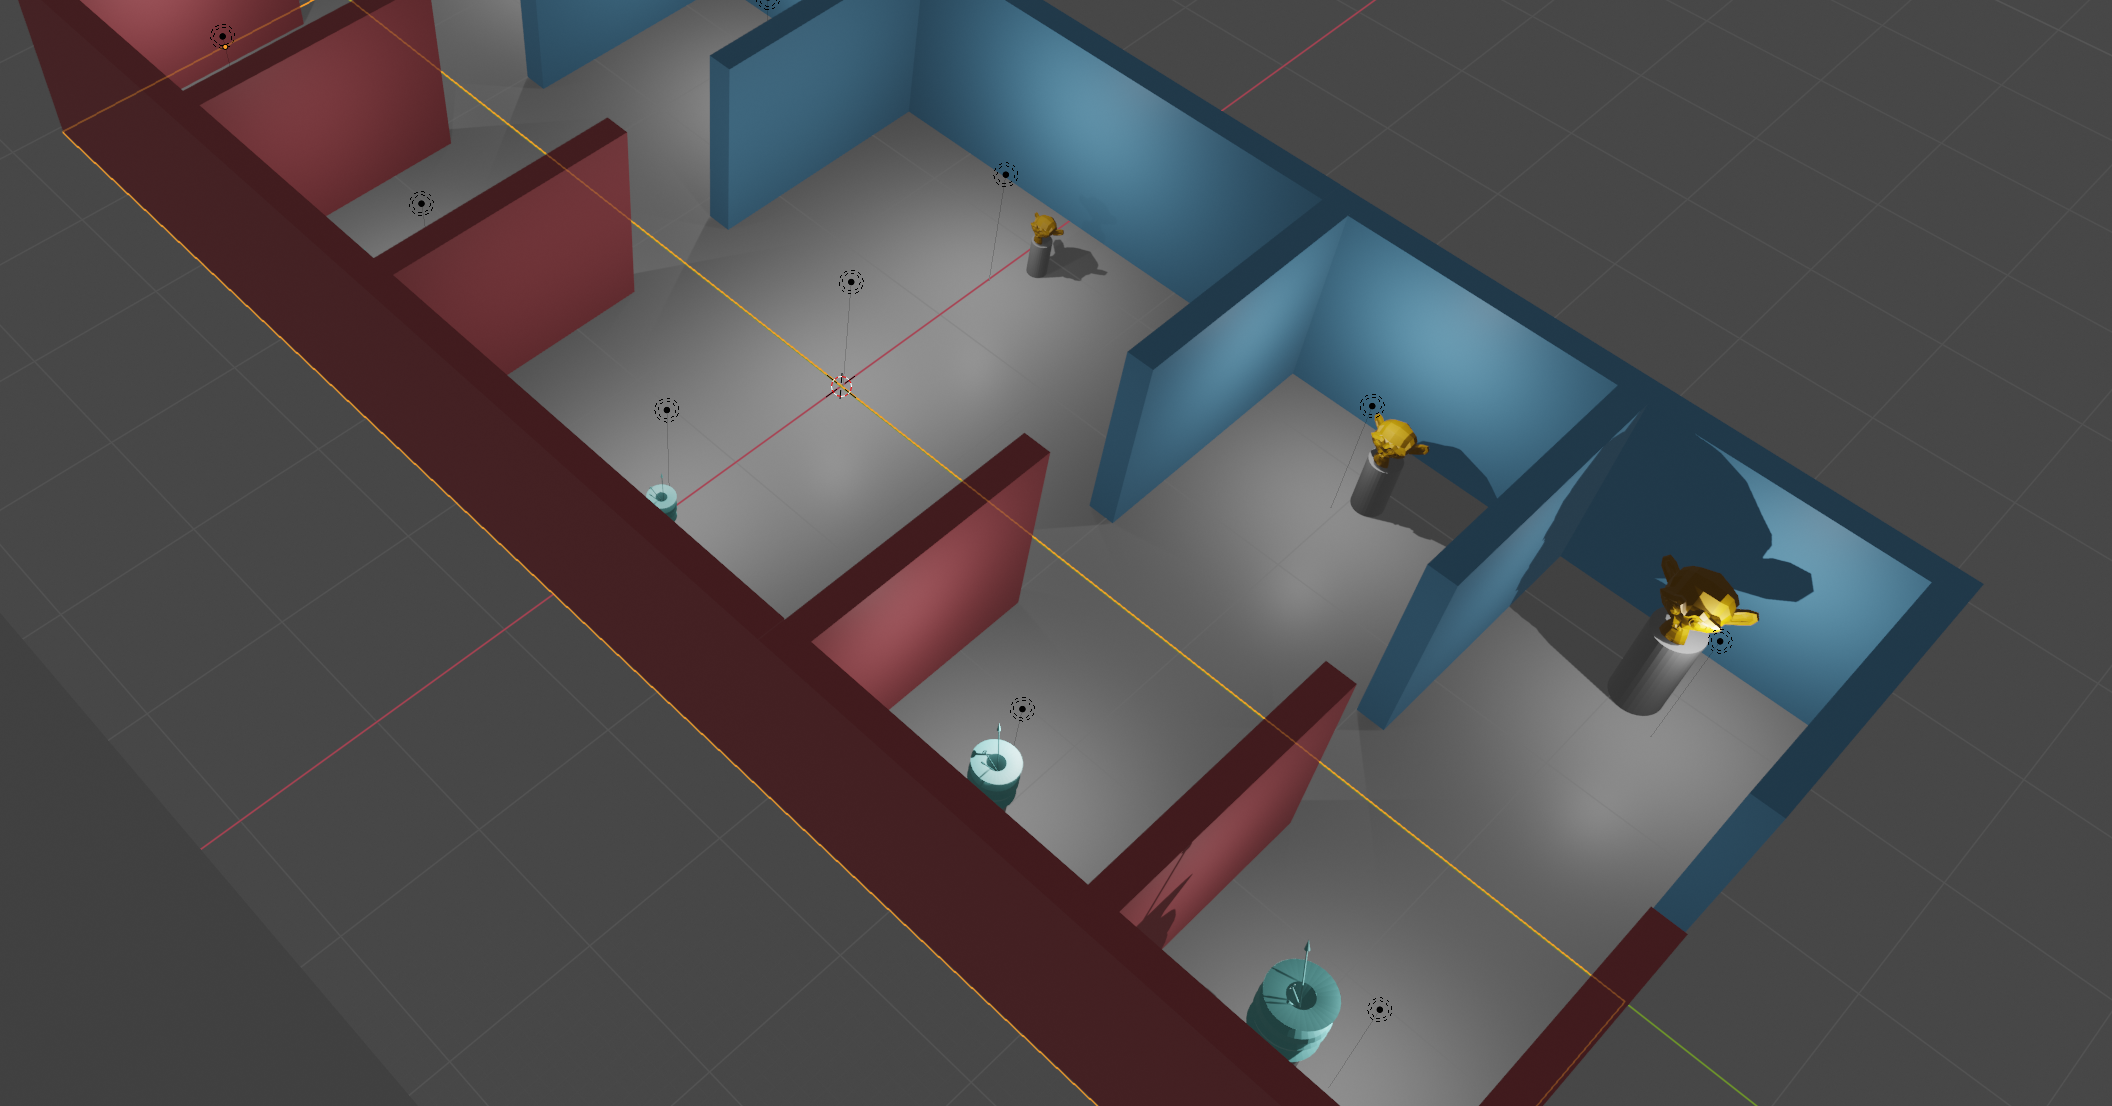
\includegraphics[width=5in]{img/implementation_generatingData_blenderSetup.png}
	\caption{The test scene for generating data. Each object is placed in a room and is separated by walls.}
	\label{pic:implementation_generatingData_blenderSetup}
\end{figure}

%[TODO: Renders and labels for example objects]
For the test objects the authors used two objects. One is a already existing monkey head in blender, the other one has been self-modelled and represents a vase with some decorating sticks in it. Both objects can be seen in Figure~\ref{pic:implementation_generatingData_testObject}.

\begin{figure*}[h!]
	\centering
	\begin{subfigure}[t]{0.4\textwidth}
		\centering
		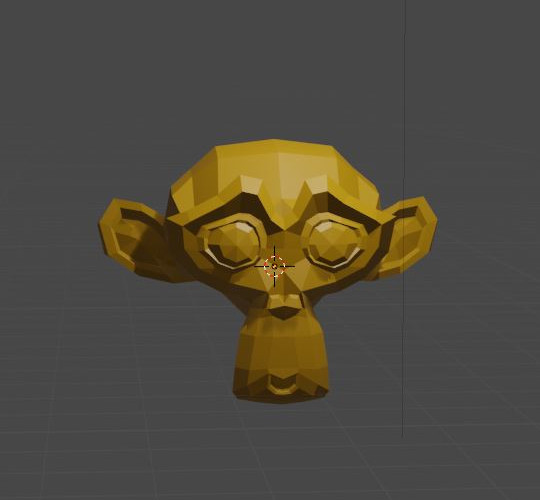
\includegraphics[width=\textwidth]{img/implementation_generatingData_testObject1.jpg}
		\caption{One of the test objects - a monkey head.}
	\end{subfigure}%
	~ 
	\begin{subfigure}[t]{0.4\textwidth}
		\centering
		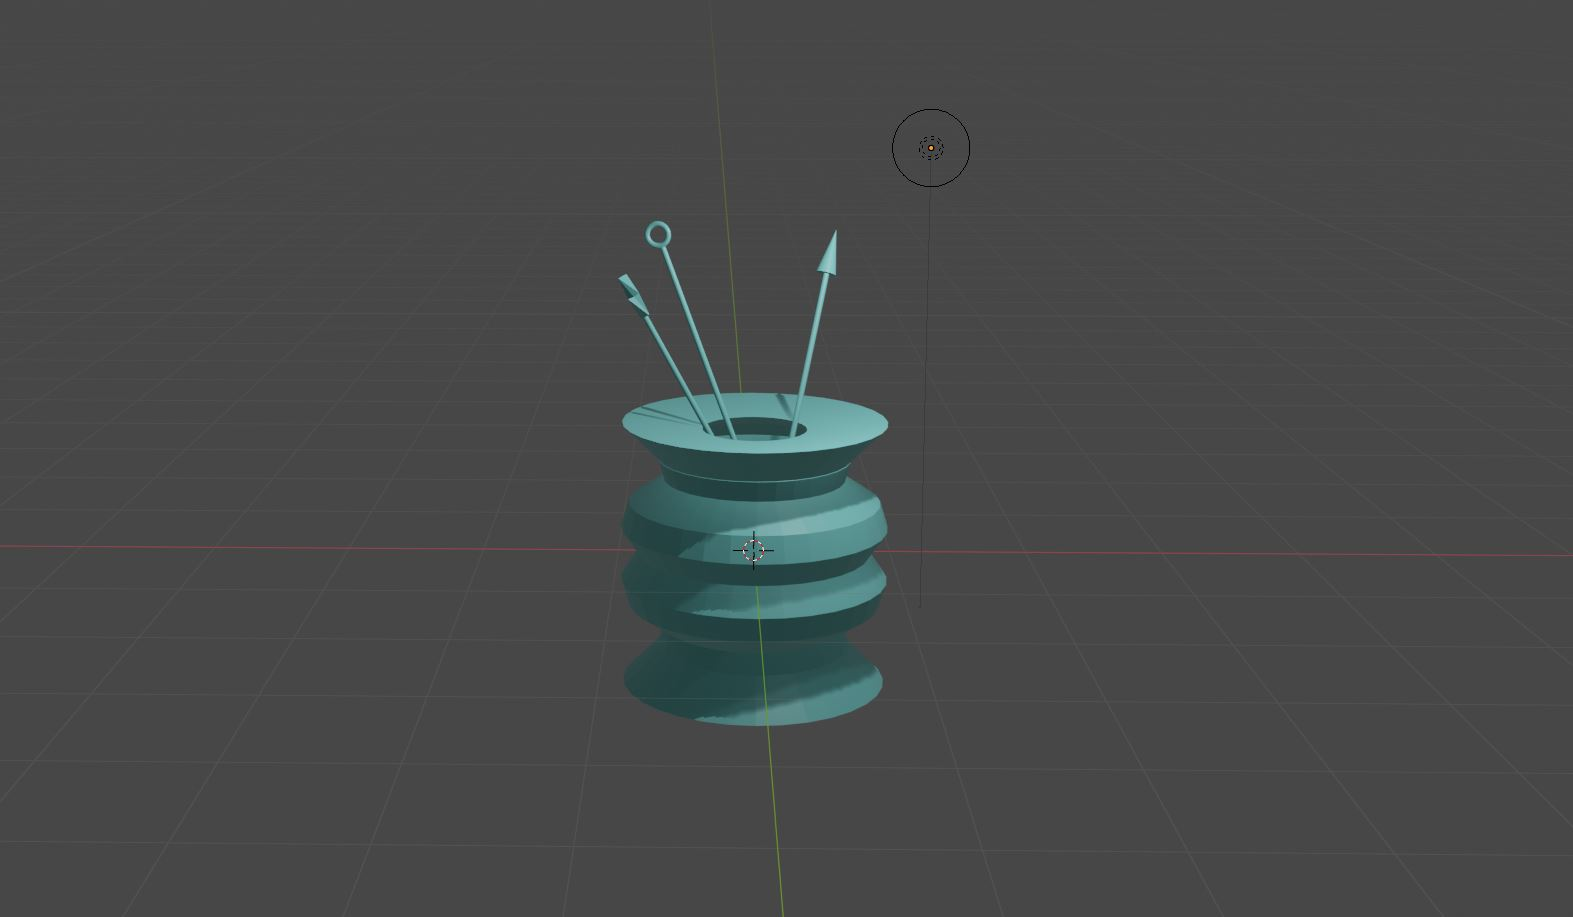
\includegraphics[width=\textwidth]{img/implementation_generatingData_testObject2.jpg}
		\caption{One of the test objects - a decorative vase.}
	\end{subfigure}
	\caption{The two test objects as displayed in the Blender interface.}
	\label{pic:implementation_generatingData_testObject}
\end{figure*}

\newpage

\subsection{Generating the Render-Pairs}
The following code generates the two needed renders for one of the test objects:

\begin{lstlisting}[language=python]
# Generate for 1 object
def generate_1(renderpath, infopath, target_name, iterations):
target_loc = bpy.data.objects[target_name].location

XMIN = target_loc.x - 0.6 if target_loc.x > 0 else target_loc.x + 0.6
XMAX = target_loc.x - 8.6 if target_loc.x > 0 else target_loc.x + 8.6
YMIN = target_loc.y - 1.85
YMAX = target_loc.y + 1.85
ZMIN = 0.75
ZMAX = 2

RENDERPATH = renderpath + target_name
INFOPATH = infopath + target_name

RENDERFILEPATH = RENDERPATH + "/{}-{}.jpg"
INFOFILEPATH = INFOPATH + "/{}-{}.txt"

make_dirs(RENDERPATH, INFOPATH)

for i in range(0, iterations):
# Calculate values
X = random.uniform(XMIN, XMAX)
Y1 = random.uniform(YMIN, YMAX)
Y2 = Y1 + 1 if (Y1 - target_loc.y) < 0 else Y1 - 1
Z = random.uniform(ZMIN, ZMAX)

# Add first camera
add_camera(X, Y1, Z, target_name)
write_dist_info(INFOFILEPATH, target_name, i, 1)
render(RENDERFILEPATH, i, 1)
del_cameras()

# Add second camera
add_camera(X, Y2, Z, target_name)
write_dist_info(INFOFILEPATH, target_name, i, 2)
render(RENDERFILEPATH, i, 2)
del_cameras()
\end{lstlisting}

This code can seem overwhelming at first, so the authors decided to explain each part of it. The first code block

\begin{lstlisting}[language=python]
target_loc = bpy.data.objects[target_name].location

XMIN = target_loc.x - 0.6 if target_loc.x > 0 else target_loc.x + 0.6
XMAX = target_loc.x - 8.6 if target_loc.x > 0 else target_loc.x + 8.6
YMIN = target_loc.y - 1.85
YMAX = target_loc.y + 1.85
ZMIN = 0.75
ZMAX = 2
\end{lstlisting}

stores the location of the given target, or object, in the variable 'target\_loc'. Relative to this location the min/max values for the X/Y/Z coordinates are being calculated. These coordinates are used for the camera placement, so the camera is placed relatively to the object. 'YMIN', for example means, that the camera's Y value can be no further than 1.85m to the left of the object. 'YMAX' clamps this value so there is a border on the right side as well.

\begin{lstlisting}[language=python]
# Calculate values
X = random.uniform(XMIN, XMAX)
Y1 = random.uniform(YMIN, YMAX)
Y2 = Y1 + 1 if (Y1 - target_loc.y) < 0 else Y1 - 1
Z = random.uniform(ZMIN, ZMAX)
\end{lstlisting}

This code block right here does exactly what described before. A random value for X/Y/Z is chosen. Notice that the Y value is split in two, where 'Y1' uses 'YMIN' and 'YMAX' and 'Y2' uses 'Y1' for calculation. This is to guarantee a different angle to the object, because camera one will use 'Y1' and the second camera will use 'Y2'.

[TODO: Maybe add image illustrating above text]

\begin{lstlisting}[language=python]
# Add first camera
add_camera(X, Y1, Z, target_name)
write_dist_info(INFOFILEPATH, target_name, i, 1)
render(RENDERFILEPATH, i, 1)
del_cameras()

# Add second camera
add_camera(X, Y2, Z, target_name)
write_dist_info(INFOFILEPATH, target_name, i, 2)
render(RENDERFILEPATH, i, 2)
del_cameras()
\end{lstlisting}

This last code block is basically the same for each camera. The first camera uses 'Y1' for its placement, centered on 'target\_name' (the object). Then, from the location of the first camera, the distance to the object is calculated and written to a file. After the calculation of the actual distance blender renders an image from the first camera's point of view, after which the first camera is being deleted. This is the same for the second camera, except it uses 'Y2' for its placement.

\section{OpenCV}
OpenCV is a framework for image manipulation. Some of its use cases are changing the colour spectrum, filtering the image by colour and cropping images. The authors use OpenCV to test whether there are differences between filters for the images in the training data, for example greyscale images compared to coloured images. An example render, which OpenCV gets as an input can be seen in Figure~\ref{pic:implementation_opencv_original}.

\begin{figure}[h!]
	\centering
	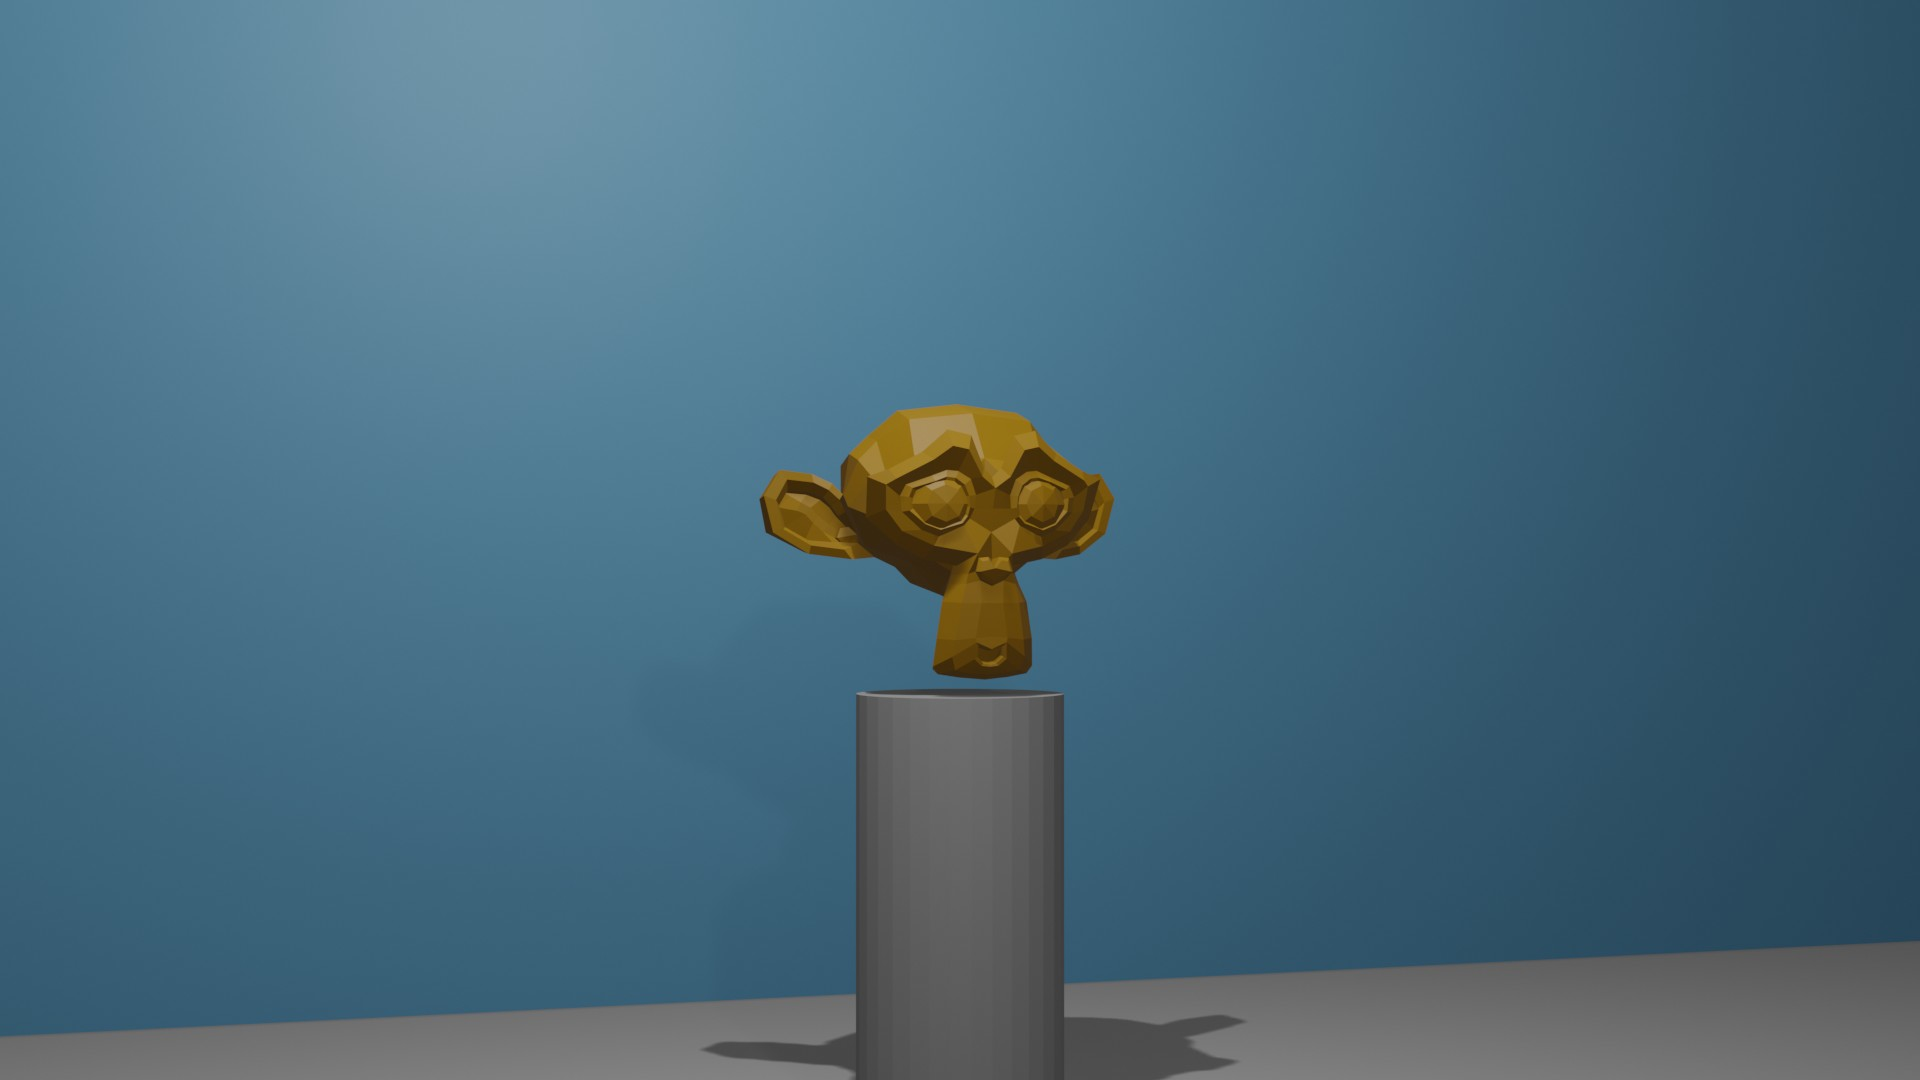
\includegraphics[width=4in]{img/implementation_opencv_original.png}
	\caption{One of two original renders produced by Blender, both depicting the same object from different points of view.}	%22_2
	\label{pic:implementation_opencv_original}
\end{figure}

\subsection{Greyscale}
Converting an image into greyscale can easily be achieved by the following OpenCV code:

\begin{lstlisting}[language=python]
import cv2

image = cv2.imread('path/to/image')
image_greyscale = cv2.cvtColor(image, cv2.COLOR_BGR2GRAY)
cv2.imwrite('path/for/saving/greyscale/image', image_greyscale)
\end{lstlisting}

This code first reads the image into 'image'. Then it converts the color of 'image' into a greyscale format and stores the result into 'image\_greyscale', which is then written to the specified path. The output generated by this code is depicted in Figure~\ref{pic:implementation_opencv_greyscale}.

\begin{figure}[h!]
	\centering
	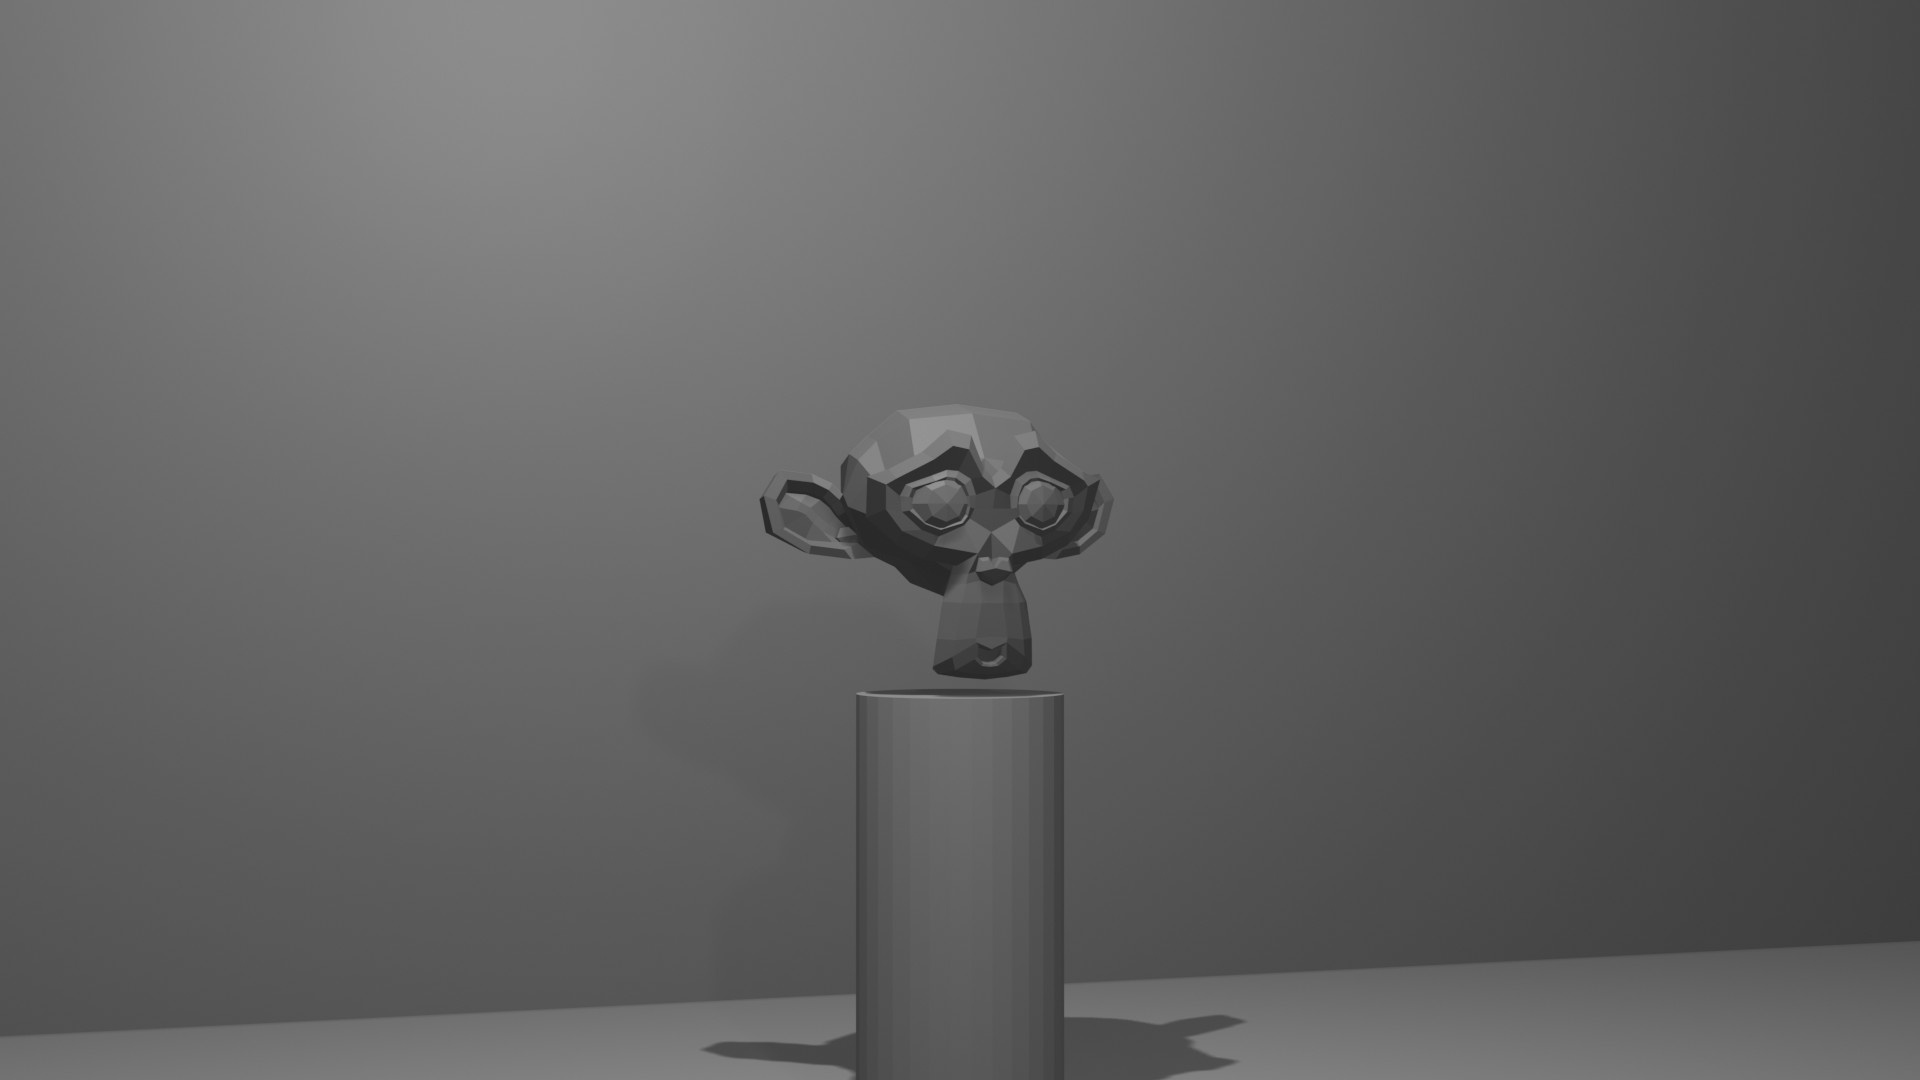
\includegraphics[width=4in]{img/implementation_opencv_greyscale.png}
	\caption{The greyscale image produced by OpenCV.}
	\label{pic:implementation_opencv_greyscale}
\end{figure}

The advantage of using greyscale images in Neural Networks is the simplification of the input layer. In greyscale images each pixel can be represented by a single decimal value between 0 and 1. This enables the first layer of the neural network to be two dimensional instead of the three dimensional counterpart, where each pixel is represented by the three decimal values for the red, green and blue colour channels.

\subsection{Resolution}
By reducing the resolution of an image the density of pixels is lessened. In this process information, that can not be regained, is lost. The OpenCV code for downscaling the images used by the authors is the following:

\begin{lstlisting}[language=python]
import cv2

image = cv2.imread('path/to/image')

scale_percent = 10  # percent of original size
width = int(image.shape[1] * scale_percent / 100)
height = int(image.shape[0] * scale_percent / 100)
dim = (width, height)

downscaled = cv2.resize(image, dim)
cv2.imwrite('{}/{}'.format(newdir_path, filename), downscaled)
\end{lstlisting}

OpenCV provides a resize function, which takes an image and the new dimensions of the image as an argument and outputs the resized image. To make sure the aspect ratio stays the same new image dimensions are calculated as a percentage of the original ones.

The output image of this code can be found in Figure~\ref{pic:implementation_opencv_resolution}.

\begin{figure}[h!]
	\centering
	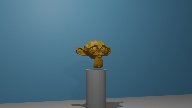
\includegraphics[width=4in]{img/implementation_opencv_resolution.jpg}
	\caption{Image with lower resolution than the original one. Due to the fact that the image is displayed in the same size as Figure~\ref{pic:implementation_opencv_original}, the pixel size in this image appears larger.}
	\label{pic:implementation_opencv_resolution}
\end{figure}

Downscaling the images before they are passed into the Neural Network can be profitable, because the number of weights in the first layer of the network is reduced. This can advance the learning speed.

\subsection{Cropping}
Cropping an image can remove unnecessary or unwanted parts of an image by simply cutting off areas. This is often wanted in photography to only keep what is interesting in a photo and to shift the view of the viewer to specific areas. However, the authors guess that cropping an image will worsen performance of the neural network, because information of the relative sizes are partly lost. It basically compares to zooming into the image.

Such a cropped image produced by the following code can be found in Figure~\ref{pic:implementation_opencv_cropping}.

\begin{lstlisting}[language=python]
import cv2

image = cv2.imread('path/to/image')

crop_margin_percent = 5
crop_margin_width = int(image.shape[1] * crop_margin_percent / 100)
crop_margin_height = int(image.shape[0] * crop_margin_percent / 100)

crop_img = image[crop_margin_width:-crop_margin_width, crop_margin_height:-crop_margin_height]
cv2.imwrite('{}/{}'.format(newdir_path, filename), crop_img)
\end{lstlisting}

\begin{figure}[h!]
	\centering
	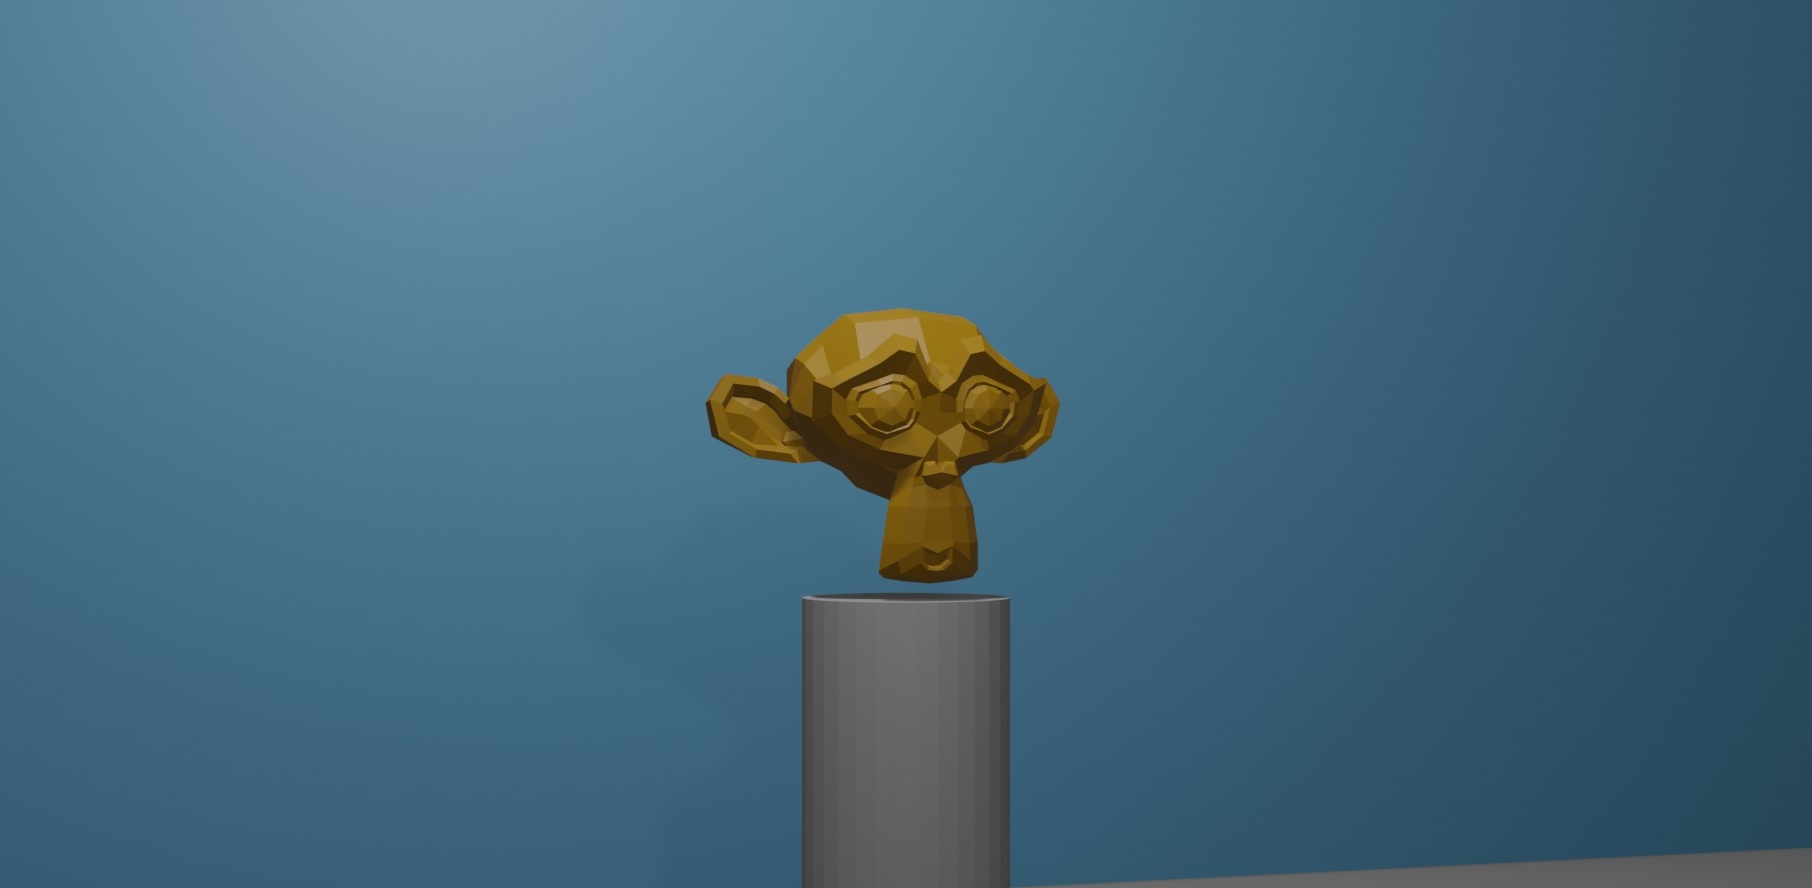
\includegraphics[width=4in]{img/implementation_opencv_cropping.jpg}
	\caption{In this image five percent of each side was removed, therefore the object appears closer if the image is displayed in the same size. Some information positioned in the outer areas of the image are lost during the cropping process.}
	\label{pic:implementation_opencv_cropping}
\end{figure}

\subsection{Saturated}
A saturated image means stronger colours, basically making them more distinguishable from each other. If an image is not saturated enough, colours appear as "washed out" and differences in colour are difficult to determine. Therefore, in order to help the neural network, the authors decided to also test with saturated versions of these images.

\begin{lstlisting}[language=python]
import cv2

image = cv2.imread('path/to/image')

hsv = cv2.cvtColor(image, cv2.COLOR_BGR2HSV).astype('float32')
(h, s, v) = cv2.split(hsv)
s *= 1.5
s = np.clip(s, 0, 255)
hsv = cv2.merge([h, s, v])
saturated = cv2.cvtColor(hsv.astype('uint8'), cv2.COLOR_HSV2BGR)
cv2.imwrite('{}/{}'.format(newdir_path, filename), saturated)
\end{lstlisting}

To saturate an image using OpenCV it has to be converted into the HSV colour representation. The HSV representation specifies each colour as a hue, a saturation and a value. Therefore changing the saturation in this model is relatively easy, as the saturation value of each pixel can simply be multiplied by a constant. Before the image can be converted back into the bgr colour representation the saturation values are restricted between 0 and 255, the lowest and highest saturation possible. The result achieved by this code can be seen in Figure~\ref{pic:implementation_opencv_saturated}.

\begin{figure}[h!]
	\centering
	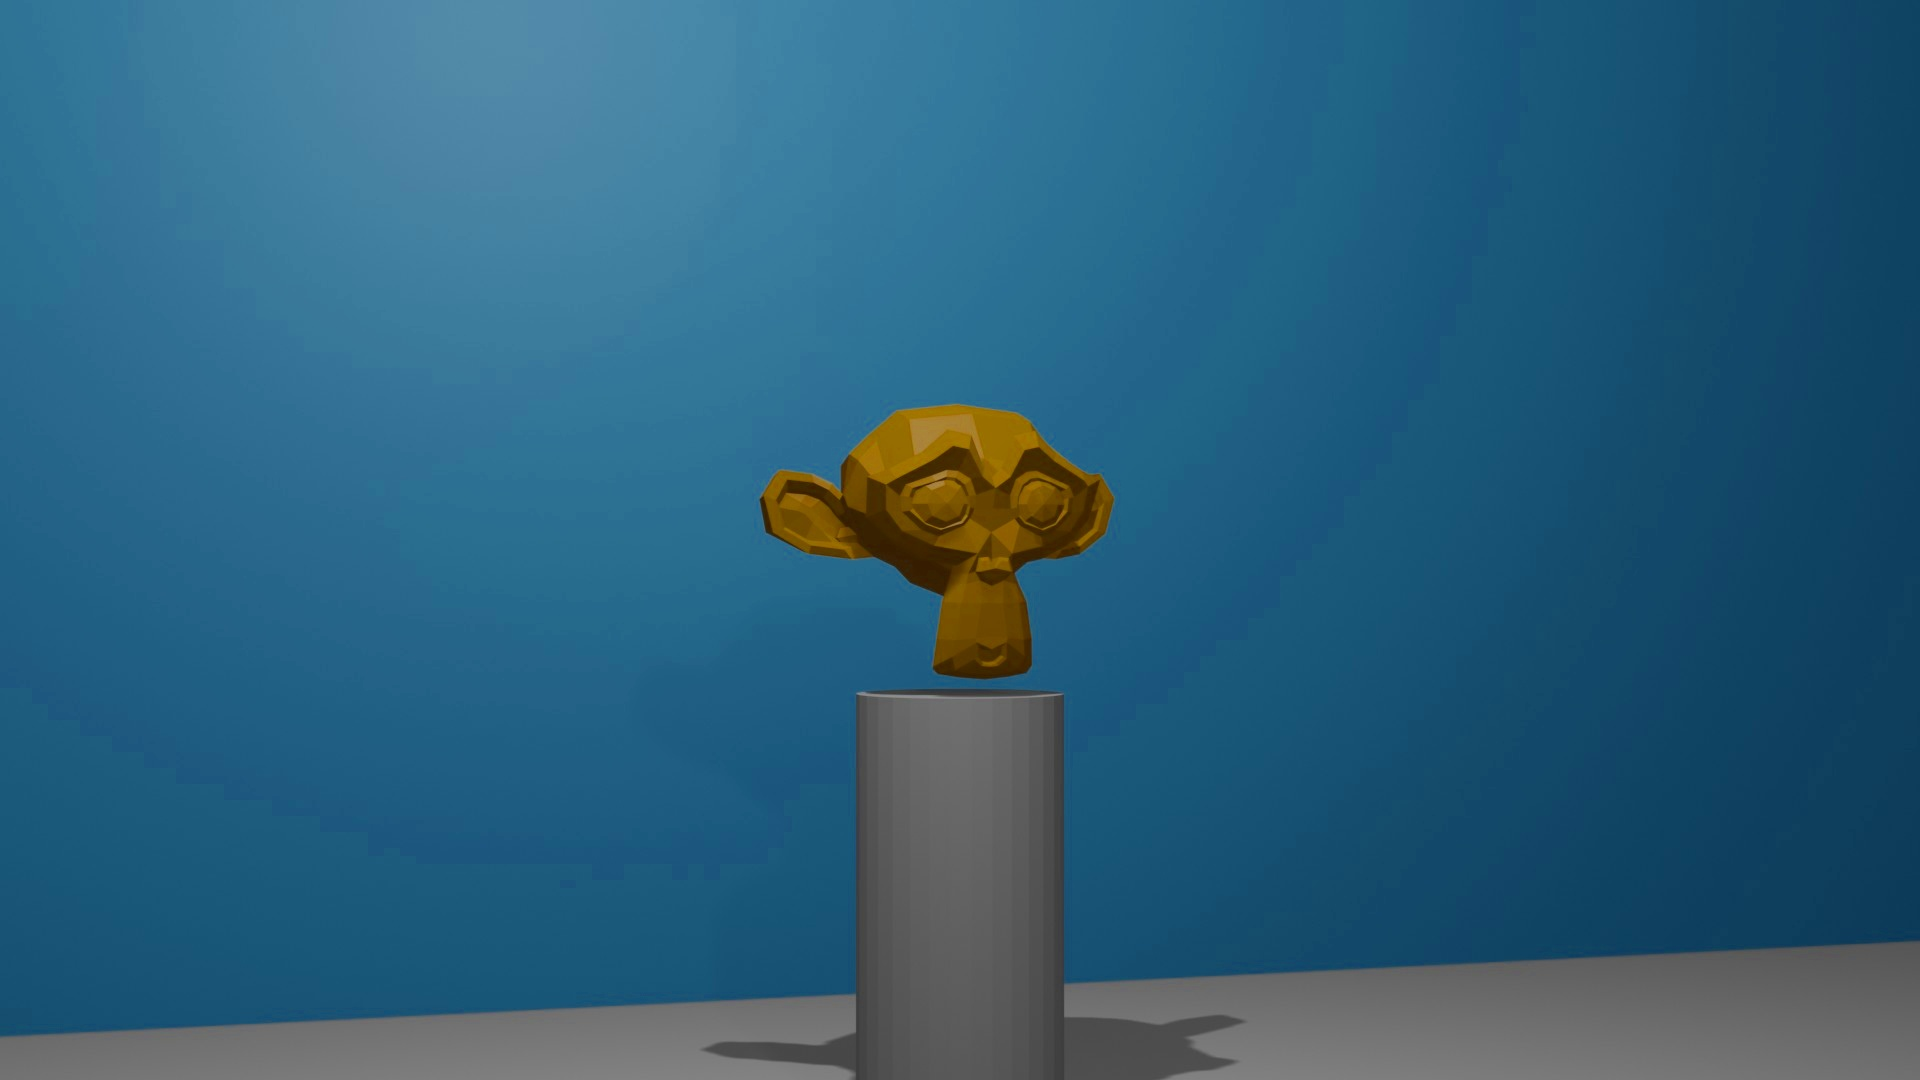
\includegraphics[width=4in]{img/implementation_opencv_saturated.jpg}
	\caption{Comparison between normal and saturated image.}
	\label{pic:implementation_opencv_saturated}
\end{figure}

\subsection{Brightness}
Because the neural network should also work in different environment, where other methods could have problems, the authors also tested with overly bright images. This makes it very hard to notice dark areas, such as shadows, to help with distances between objects and scaling of objects.

\begin{lstlisting}[language=python]
import cv2

image = cv2.imread('path/to/image')

alpha = 1  # contrast
beta = 60  # brightness
bright_img = cv2.convertScaleAbs(image, alpha=alpha, beta=beta)

cv2.imwrite('{}/{}'.format(newdir_path, filename), bright_img)
\end{lstlisting}

\begin{figure}[h!]
	\centering
	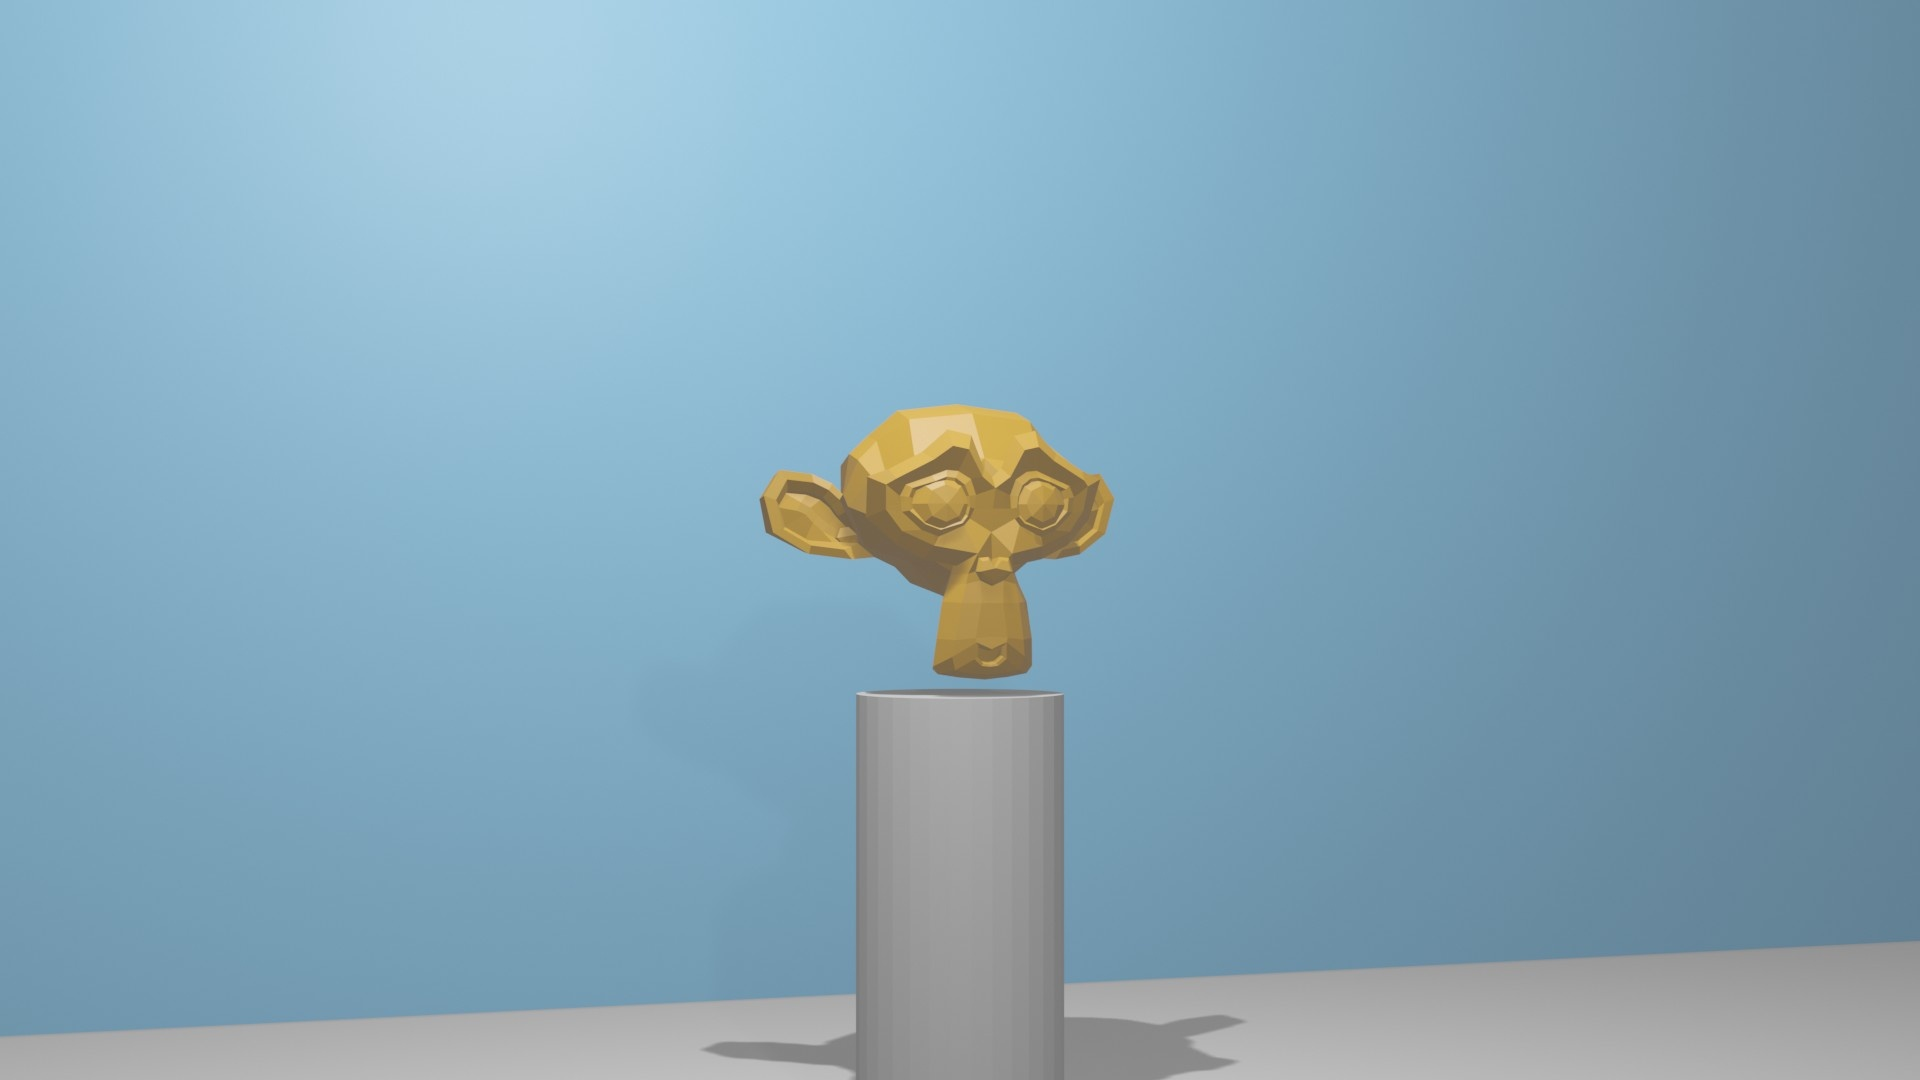
\includegraphics[width=4in]{img/implementation_opencv_brightness.jpg}
	\caption{The original image (Figure~\ref{pic:implementation_opencv_original}) modified by the brightening code. The image appears more washed out, as all colours are move similar due to them having moved closer to white.}
	\label{pic:implementation_opencv_brightness}
\end{figure}

\section{Neural Network}
\subsection{Setting up the Neural Network}
Using Python and TensorFlow enabled the authors to exchange the components of the neural network without much effort. This enabled a fast development of a working prove of concept. The structure of the neural network depicted in Figure~\ref{pic:implementation_neuralNetwork_testringTheStructureOfTheNeuralNetwork_model} was the first one tested and already proved effective.

\begin{figure}[h!]
	\centering
	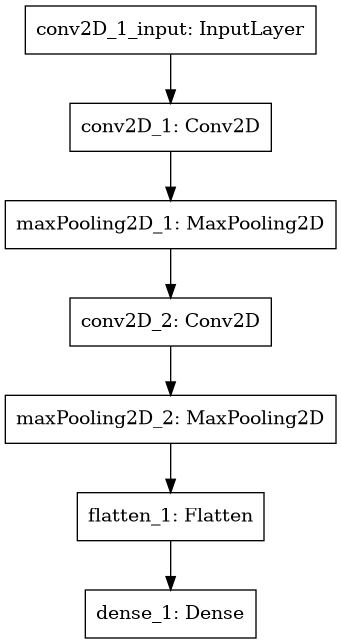
\includegraphics[width=2in]{img/implementation_neuralNetwork_testringTheStructureOfTheNeuralNetwork_model.png}
	\caption{A sequential model of a neural network. The input layer receives the greyscale images. The image is then processed by two convolutional layers, each followed by a max pooling layer reducing the width in one dimension and therefore reducing the number of weights. The last layer, a dense layer, outputs the number representing the normalized distance the neural network estimated. The input of this dense layer is a unrolled version of the output of the last max pooling layer. This is achieved by the flatten layer.}
	\label{pic:implementation_neuralNetwork_testringTheStructureOfTheNeuralNetwork_model}
\end{figure}

In the first test run only 50 greyscale images where used. This encourages overfitting and was only intended to test if the neural network was syntactically set up correctly. At this point in time the first problem arose. The accuracy from the beginning always was one, meaning that the distance to the object in all images was estimated correctly, which does not seem plausible. Even if the neural network was overfitted at least in the beginning the accuracy should be less than one.

It appeared later that this was due to the fact, that the true as well as the estimated output values were not normalized. In a neural network the output of each node has to be between zero and one. As all true values (the distance to the object outputted by Blender) where above one they where simply converted to a value of one. The neural network was trained to only output one, which it easily managed to do, and therefore received an accuracy of one.

Normalizing the distances was a simple task as the maximum distance in the generated images was 10 meters. Therefore simply dividing by the maximum possible value reduced the range of the values into the normalized form. This however had the consequence that the accuracy of the neural network was zero, however long it was trained.

At this point it is noteworthy that in machine learning one can distinguish between classification and regression problems. In classification problems the output value can only be one of a discrete set of values. For example image classification, where a machine learning algorithm labels images as either depicting a cat or a dog. In this example two possible output values are defined. Regression problems however are identified by the output value being able to take any continuous value. The distance estimation problem the described in this thesis is a regression problem, as the distance to the object can be any value between zero and ten.

Accuracy is a system of measurement which describes how often the machine learning algorithm ``guessed'' the correct output. If the output differs in the last decimal place (in our case less than a nano meter) the accuracy does not get increased. Therefore accuracy is only used in classification problems, where the accuracy gets increased for example for correctly guessing that an image depicts a cat (the output matching the actual value exactly). The equivalent used in regression problems is called metric. The metric chosen by the authors is the mean absolute percentage error. It represents a difference between the actual and the output value as a percentage. The lower this percentage the better the performance of the neural network.

As an optimizer the authors chose stochastic gradient descent as the other optimizers available in TensorFlow are only variations of this optimizer.

After these modifications the output seemed plausible enough to increase the number of training images from 50 to 10000. Up to this point all images where loaded and converted into tensors before the actual training began. This posed no problem when loading 50 images, however loading 10000 images was not possible with the limited RAM installed on the machine. Since the process was running on a Linux machine, the kernel killed the process due to resource starvation.

The most obvious solution was to split the images into smaller sections and only load and process one of these batches at a time. Additionally the authors chose to store the computed weights after each of these batches, enabling the user to stop the training at any given point in time and still have the relatively new weights stored. When starting the program again, the weights are loaded and training can resume.

\subsection{First results}
The first serious training run was performed on 2500 binocular images of a single object. Therefore it was expected, that the neural network would overfit and not work on any other objects. The setup of layers chosen was the one depicted in Fig.~\ref{pic:implementation_neuralNetwork_testringTheStructureOfTheNeuralNetwork_model}.

While training the loss sank from around 210,000,000 after having ``seen'' 50 images to a value of fluctuating between 0.21 and 0.27 while the mean absolute percentage error sank from around 11,000,000,000\% to a value fluctuating between 11.1\% and 16.5\%.

The weights of this trained neural network are visualized in Fig.~\ref{pic:implementation_neuralNetwork_structureOfOurNeuralNetwork_weights}. While interpreting weights of a neural network is a vague science, some features of these weights are worth mentioning. For example a few of the matrices shown in Subfig.~\ref{pic:implementation_neuralNetwork_structureOfOurNeuralNetwork_weights_a} have a dark blue blob appear in the upper middle part, while the bottom left and right pixels show the brightest colours. Since brighter colours mean more influence of the input value received, the authors guess, that the size of objects could be determined by these convolution windows. These convolution windows could for example react to the size of the mount of the object, which is located in the lower part of the image. The second subfigure (Subfig.~\ref{pic:implementation_neuralNetwork_structureOfOurNeuralNetwork_weights_b}) is hard to interpret, as the tensors are already quite abstract at this point. The dense layer (Subfig.~\ref{pic:implementation_neuralNetwork_structureOfOurNeuralNetwork_weights_c}), however, gives a low weight to most input values, only using some for the calculation of the final output. Even more interesting are the horizontal stripes appearing in the weights of the dense layer. To get a better understanding of why these stripes appear the authors decided to group the weights of this layer into the sizes of the output of the last convolutional layer. The resulting image can be found in Subfig.~\ref{pic:implementation_neuralNetwork_structureOfOurNeuralNetwork_weights_d}. From this it is apparent, that the neural network is able to work out that the input image consists of two separate renders. Most of these units focus on the two middle part of the two images separately, some on a larger a region, while other only on the exact place where the object is located. Only few units focus on the section where the shadow of the object is located.

\newpage

\begin{figure*}[h!]
	\centering
	\begin{subfigure}[t]{0.585\textwidth}
		\centering
		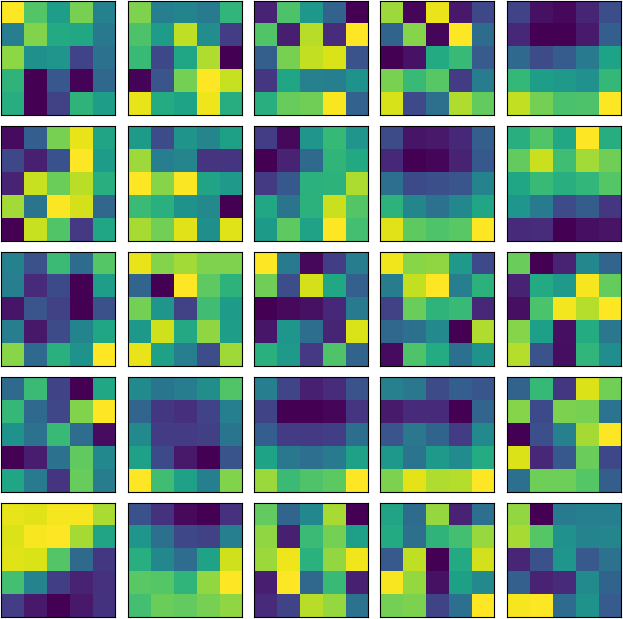
\includegraphics[width=\textwidth]{img/implementation_neuralNetwork_structureOfOurNeuralNetwork_conv2D_1.png}
		\caption{The already trained weights of the first convolutional layer. Each of the 5x5 pixel matrices displays the weights of one layer of the convolution window.}
		\label{pic:implementation_neuralNetwork_structureOfOurNeuralNetwork_weights_a}
	\end{subfigure}
	~
	\begin{subfigure}[t]{0.585\textwidth}
		\centering
		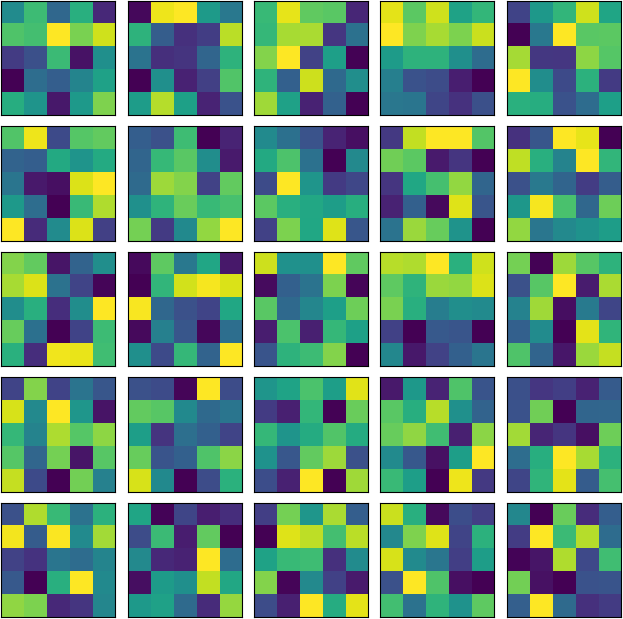
\includegraphics[width=\textwidth]{img/implementation_neuralNetwork_structureOfOurNeuralNetwork_conv2D_2.png}
		\caption{The trained weights of the second convolutional layer. Again each of the 5x5 pixel matrices displays the weights of one layer of the second convolution window.}
		\label{pic:implementation_neuralNetwork_structureOfOurNeuralNetwork_weights_b}
	\end{subfigure}
	~
	\begin{subfigure}[t]{0.385\textwidth}
		\centering
		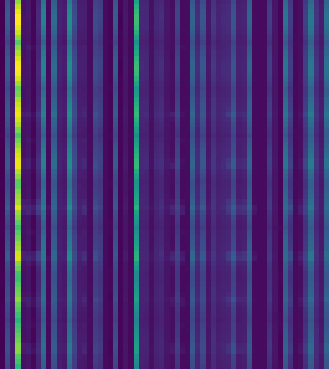
\includegraphics[width=\textwidth]{img/implementation_neuralNetwork_structureOfOurNeuralNetwork_dense_1.png}
		\caption{The trained weights of the dense layer, which outputs the estimated result. Horizontal stripes appear because the one dimensional weight vector is displayed as a 72x64 matrix for convenience.}
		\label{pic:implementation_neuralNetwork_structureOfOurNeuralNetwork_weights_c}
	\end{subfigure}
	~
	\begin{subfigure}[t]{\textwidth}
		\centering
		
\includegraphics[width=\textwidth]{img/implementation_neuralNetwork_structureOfOurNeuralNetwork_dense_1b.png}
		\caption{The same weights as in Subfig.~\ref{pic:implementation_neuralNetwork_structureOfOurNeuralNetwork_weights_c} regrouped into 64 4x18 units.}
		\label{pic:implementation_neuralNetwork_structureOfOurNeuralNetwork_weights_d}
	\end{subfigure}
	\caption{In all subplots the highest value occurring in a unit of pixels is displayed as a yellow colour and the lowest value occurring is a dark blue colour. All other values are shown as the corresponding colours ranging from yellow over green to dark blue.}
	\label{pic:implementation_neuralNetwork_structureOfOurNeuralNetwork_weights}
\end{figure*}

\newpage

\subsection{Modifications to the Neural Network}
Since the authors wanted to reach an accuracy of $\pm 10\%$ and the first test only performed with an accuracy of around $\pm 13\%$ possible modifications to the neural network where tested. One of these settings is the number of epochs. This controls how often the input data is looped through. E.g. setting the number of epochs to three makes the fit method go through all input images three times. As it turned out increasing the number of epochs does not have any measurable affects on the performance. Therefore the value was set to a count of two epochs.

The next change to the structure of the neural network was the introduction of a momentum term. A momentum term helps to avoid getting stuck in a local, but not the lowest, minimum. One can imagine the optimizer as a mechanism which lets a sphere ``roll'' down a surface to find the minimum value. A two dimensional version of this is visualized in Fig.~\ref{pic:implementation_neuralNetwork_modificationsToTheNN}. When no momentum term is defined training behaves as if the sphere had no inertia, which can lead to it getting stuck in a valley, which is not the lowest reachable point. When inertia is added the change in the position of the sphere depends not only on the gradient of the curve in the current position of the sphere, but also on the last few gradients the sphere ``rolled'' along. Therefore the sphere in Subfig.~\ref{pic:implementation_neuralNetwork_modificationsToTheNN_b} manages to find a lower minimum of the curve.

\begin{figure*}[h!]
	\centering
	\begin{subfigure}[t]{0.5\textwidth}
		\centering
		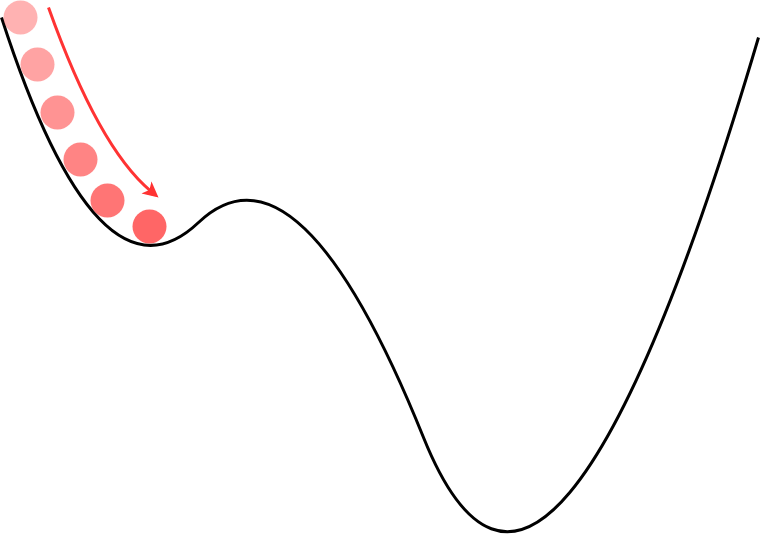
\includegraphics[width=\textwidth]{img/implementation_neuralNetwork_modificationsToTheNN_a.png}
		\caption{Visualization of the optimization without a momentum term. The red sphere gets stuck in a local minimum, but fails to find the lowest possible point reachable.}
		\label{pic:implementation_neuralNetwork_modificationsToTheNN_a}
	\end{subfigure}%
	~
	\begin{subfigure}[t]{0.5\textwidth}
		\centering
		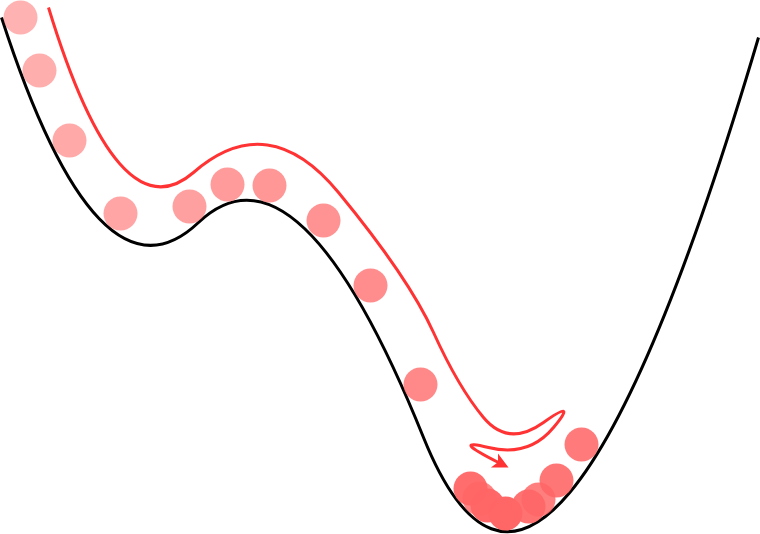
\includegraphics[width=\textwidth]{img/implementation_neuralNetwork_modificationsToTheNN_b.png}
		\caption{Visualization of the optimization with a momentum term defined. Here the red sphere has enough inertia to ``roll'' over the small bump, which enables it to reach the lower local minimum.}
		\label{pic:implementation_neuralNetwork_modificationsToTheNN_b}
	\end{subfigure}
	\caption{Two figures showing representations of optimization functions. In both cases the optimisation is complete when the red sphere reached a local minimum. The difference in the figures is the use of a momentum term.}
	\label{pic:implementation_neuralNetwork_modificationsToTheNN}
\end{figure*}



\section{C++ Implementation}

\section{Technical difficulties}

\filbreak
